

\section{Experiments}
\label{sec:experiments}

\subsection{Dataset and Metrics}
\textbf{Dataset.} We test on three online action detection datasets. \emph{THUMOS'14}~\cite{THUMOS14} consists of over 20 hours of sports video annotated with 20 actions. \emph{TVSeries}~\cite{oad2016} includes 27 episodes of 6 popular TV series, about 150 minutes each and 16 hours total. \emph{HDD}~\cite{hdd} is a large-scale human driving video dataset comprising 104 hours of untrimmed videos and 11 action categories. Furthermore, we evaluate on \emph{EpicKitchens-100}~\cite{ek100} that contains 100 hours of egocentric videos with at least 90K action segments and whose narrations are mapped to 97 verb classes and 300 noun classes.


\textbf{Evaluation Metrics.} For online action detection, following previous works \cite{oad2016, LAP-Net, oadtr, lstr, colar}, we use per-frame \emph{mean Average Precision (mAP)} on THUMOS'14 and HDD, and per-frame \emph{mean calibrated Average Precision (mcAP)}~\cite{oad2016} on TVSeries. For action anticipation, we employ \emph{Top-5 Verb/Noun/Action Recall}  to measure the performance with an anticipation period $\tau = 1s$~\cite{ek100}.




\subsection{Implementation details} 
Following prior works~\cite{trn, lstr, testra}, we conduct our experiments on pre-extracted features. For TVSeries and THUMOS'14, we first resample the videos at 24 FPS and then extract the frames at 4 FPS for training and validation. We adopt a two-stream network~\cite{tsn} to extract feature.  
We use off-the-shell checkpoint released by mmaction2~\cite{mmaction2} that pretrained on ActivityNet v1.3 \cite{anet} and Kinetics \cite{kinetics} to extract frame-level RGB and optical features. On EK100, following~\cite{rulstm}, we resample the videos at 30 FPS and then fine-tune the two-stream TSN on the classification task.


\textbf{Memory Dropping.}
Despite the promising capabilities of the dense attention mechanism, capturing long-range dependencies remains a challenge.
However, relying on the dense attention mechanism may lead to sub-optimization of the network, resulting in a locally optimal solution. 
We seek to explore memory-dropping strategies for implementing sparse attention during training.
We experiment with various approaches, including dropout~\cite{dropout}, top-k selection~\cite{knn}, and token dropping~\cite{mae}. We compare these strategies, recorded in the supplementary material, and find that the top-k selection yields the best performance.

\begin{table}[t]
    \centering
    \small
    \setlength{\tabcolsep}{1.0mm}{
    \begin{tabular}{cccccccccc}
    % \toprule
     % &long-term & short-term & future & interaction & $N_t$ & mAP \\
     &long & short & future & interaction & $N_t$ & detection & anticipation \\
    \midrule
    \rowcolor{smooth}
    (a) &  &  &  & - & - & 67.6$_{\textcolor{dg}{+0.0}}$ & 53.7$_{\textcolor{dg}{+0.0}}$ \\
    (b)  & & \checkmark &  & CA & 1 &  68.3$_{\textcolor{dg}{+0.7}}$ & 54.7$_{\textcolor{dg}{+1.0}}$\\
   (c) & \checkmark & \checkmark &  & CA & 1 & 68.9$_{\textcolor{dg}{+1.3}}$  & 55.3$_{\textcolor{dg}{+1.6}}$ \\
    (d) &\checkmark &  & \checkmark & CA & 1 & 68.6$_{\textcolor{dg}{+1.0}}$ & 55.8$_{\textcolor{dg}{+2.1}}$\\
    (e) & & \checkmark & \checkmark & CA & 1 & 69.2$_{\textcolor{dg}{+1.6}}$ & 56.1$_{\textcolor{dg}{+2.4}}$\\
    \hline
   (f) & \checkmark & \checkmark & \checkmark & Avg\&Cat & 1 & 68.3$_{\textcolor{dg}{+0.7}}$ & 55.3$_{\textcolor{dg}{+1.6}}$\\
   % (g) & \checkmark & \checkmark & \checkmark & CA & 0 & 67.8\\
  (g)& \checkmark&\checkmark &\checkmark & CA & 1 &  69.9$_{\textcolor{dg}{+2.3}}$ & 56.6$_{\textcolor{dg}{+2.9}}$\\
    \rowcolor{light}
  (h) &\checkmark &\checkmark &\checkmark & CA & 2 & \textbf{70.4$\bf{_{\textcolor{dg}{+2.9}}}$} & \textbf{57.3$_{\textcolor{dg}{+3.6}}$} \\
  (i) &\checkmark &\checkmark &\checkmark & CA & 3 & 70.2$_{\textcolor{dg}{+2.6}}$ &  57.1$_{\textcolor{dg}{+3.4}}$ \\
    % \bottomrule
    \end{tabular}}
    \caption{\textbf{Ablation study} on the information stream, interaction method, and times for Conditional Circular Interaction. The \sethlcolor{smooth}\hl{shallow gray row} denotes the baseline setting without any interaction.}
    \vspace{-3mm}
    \label{tab: interaction}
\end{table}

\textbf{MixClip+.}
TesTra~\cite{testra} proposed an augmentation technique called MixClip to solve over-fitting caused by large long-term memory. 
Unlike long-term memory which presents an abstract concept, short-term memory provides a continuous motion trend, often playing a decisive role in anticipation. It leads to the fact that MixClip damages the continuity of motion, thereby, does not apply to short-term memory. We propose MixClip+ to solve the issue. Due to space limitations, we will describe this part in the supplementary material.


In addition to mixing augmentation for long-term memory, we mix each feature token of short-term memory with a random clip from different videos. To maintain the continuity of short-term memory, we adopt soft fusion with hyper-parameter $\alpha = 0.25$ to mix features and the corresponding labels, similar to Mixup~\cite{mixup}. 


\subsection{Ablation Study}
\label{sec:ablation}

Now we analyze the MAT model, using the two-stream features pretrained on ActivityNet v1.3 and THUMOS'14 test set as the test bed. Furthermore, we also study the contribution of the proposed MixClip+ on EPIC-Kitchens-100.





\textbf{Segment Number.}
We evaluate the effect of segment number $N_s$ for long-term memory compression in Table~\ref{tab:segment}. We find even a small $N_s$ can improve performance, compared with two-stage compression~\cite{lstr}. However, too many segments result in too little information within each segment to effectively capture temporal dependency. We use $ N_s = 8$ as the default in the following ablation experiments.



\begin{figure}[t]
    \centering
    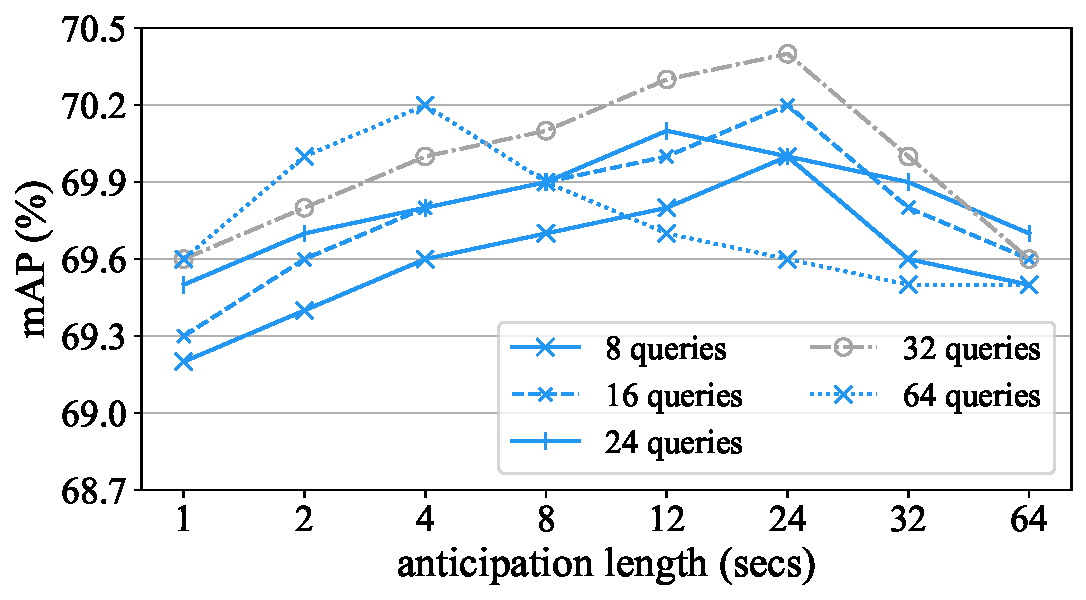
\includegraphics[width=0.45\textwidth]{images/new_query_length.pdf}
    
    \caption{\textbf{Generating latent anticipation} with different anticipation length $T_F$ and numbers of learnable tokens $N_F$.}
    \vspace{-3mm}
    \label{fig:query_length}
\end{figure}


\textbf{Query Number and Anticipation Length.}
Fig~\ref{fig:query_length} compares generating latent anticipation using $N_F$ learnable tokens with different anticipation lengths $T_F$. The experimental results indicate that, for $T_F \leq 4$, a larger $N_F$ yields superior results owing to strongly correlated semantics of short-term memory and short-term anticipation thus, the model can benefit from more tokens.
We observe that $N_F=8, 16, 32$ exhibits a similar trend in the accuracy curve, with the model achieving optimal performance with $N_F=32$. This suggests that long-term anticipation is more adaptable for sparse tokens. The observations imply that anticipation is also suitable for long- and short-term modeling.



\textbf{Future Queries Renewal.}
As Section~\ref{decoder} outlines, renewing future queries before the initial interaction improves performance. In Table~\ref{tab:renew}, we compare different renewing times (``0'' denotes no renewal and utilizes $F_A$). A plausible explanation is that, in the first interaction process, the interaction from anticipation to memory adjusts the old memory, causing its domain to shift largely, which leads to insufficient interaction from the new memory to the initial anticipation feature.

\begin{table*}[t]
    \centering
    \small
    \setlength{\tabcolsep}{2.5mm}{
    \begin{tabular}{lcccc>{\columncolor{light}}ccccccc}
     % \toprule
        \multirow{2}{*}{Method} & \multirow{2}{*}{Modality} & \multirow{2}{*}{Init} & \multicolumn{3}{c}{Overall} & \multicolumn{3}{c}{Unseen} & \multicolumn{3}{c}{Tail} \\
        \cmidrule(lr){4-6} \cmidrule(lr){7-9} \cmidrule(lr){10-12}
         & & & Verb & Noun & \cellcolor{white}Action & Verb & Noun & Action & Verb & Noun & Action \\
         \midrule
         RULSTM~\cite{rulstm} & \multirow{6}{*}{RGB} & IN-1K & 27.5 & 29.0 & 13.3 & 29.8 & 23.8 & 13.1 & 19.9 & 21.4 & 10.6 \\
         AVT~\cite{avt} &  & IN-1K & 27.2 & 30.7 & 13.6 & - & - & - & - & - & - \\
         AVT~\cite{avt} &  & IN-21K & 30.2 & 31.7 & 14.9 & - & - & - & - & - & - \\
         DCR~\cite{dcr} & & IN-1K & 31.0 & 31.1 & 14.6 & - & - & - & - & - & - \\
         TeSTra~\cite{testra} &  & IN-1K & 26.8 & 36.2 & 17.0 & 27.1 & 30.1 & \textbf{13.3} & 19.3 & 28.6 & 13.7 \\
         % \hline
         % MAT (Ours) &  & IN-1K & \textbf{30.8} & \textbf{39.1} & \textbf{18.4} & 29.3 & \textbf{30.2} & 12.1 & \textbf{23.3} & \textbf{33.1} & \textbf{15.7} \\
         MAT (Ours) &  & IN-1K & \textbf{32.7} & \textbf{39.7} & \textbf{18.8} & \textbf{31.7} & \textbf{32.1} & 12.7 & \textbf{25.7} & \textbf{32.4} & \textbf{16.0} \\
         \hline
         RULSTM~\cite{rulstm} & \multirow{4}{*}{{RGB + OF + OBJ}} & IN-1K & 27.8 & 30.8 & 14.0 & 28.8 & 27.2 & 14.2 & 19.8 & 22.0 & 11.1 \\
         TempAgg~\cite{tempagg} &  & IN-1K & 23.2 & 31.4 & 14.7 & 28.0 & 26.2 & \textbf{14.5} & 14.5 & 22.5 & 14.8 \\
         AVT+~\cite{avt} &  & IN-1K & 25.5 & 31.8 & 14.8 & 25.5 & 23.6 & 11.5 & 18.5 & 25.8 & 12.6 \\
         AVT+~\cite{avt} &  & IN-21K & 28.2 & 32.0 & 15.9 & 29.5 & 26.0 & 12.8 & 23.2 & 29.2 & 14.1 \\
        % \arrayrulecolor{light} \cmidrule(r){1-2} 
        \hline
         TeSTra~\cite{testra} & \multirow{2}{*}{RGB + OF} & IN-1K & 30.8 & 35.8 & 17.6 & 29.6 & 26.0 & 12.8 & 23.2 & 29.2 & 14.2 \\
        MAT (Ours) & & IN-1K & \textbf{35.0} & \textbf{38.8} & \textbf{19.5} & \textbf{32.5} & \textbf{30.3} & 13.8 & \textbf{28.7} & \textbf{33.1} & \textbf{16.9}  \\
    \arrayrulecolor{black}
   % \bottomrule
    \end{tabular}
    }
    \caption{\textbf{Comparison to prior work on EPIC-Kitchens-100 Action Anticipation~\cite{ek100}.} 
Accuracy measured by class-mean recall@5(\%) following the standard protocol.}
    \vspace{-3mm}
    \label{tab:ek100_anticipation}
\end{table*}

\begin{table}[t]
    \centering
    \small
    \setlength{\tabcolsep}{1.2mm}{
    \begin{tabular}{lcccccc}
     % \toprule
         Modality & Encoder & Init & FT & Overall & Unseen & Tail \\
         \midrule
    RGB & TSN & IN-1K & \checkmark & 18.8 & 12.7 & 16.0 \\
    RGB + OF & TSN & IN-1K & \checkmark & 19.5 & 13.8 & 16.9 \\
    RGB & ViT-L & K400 & & 19.1 & 16.2 & 16.1 \\
    % RGB & ViT-L & K700 & & 21.7 & 19.1 & 18.6 \\
    RGB (V) & ViT-L & Ego4D & & 21.9 & 19.4 & 18.5 \\
    RGB (N) & ViT-L & Ego4D & & 24.2 & 21.4 & 20.9 \\
    RGB (V + N) & ViT-L & Ego4D & & 24.6 & 21.4 & 21.2 \\
    \arrayrulecolor{black}
   % \bottomrule
    \end{tabular}
    }
    \caption{\textbf{Exploring different visual encoders} for EK100 action anticipation. V or N denotes the encoder is pretrained on verb or noun subset~\cite{internvideo}. ``FT'' is that the encoder is fine-tuned on the classification task of EK100.}
    \label{tab:pretrain}
    \vspace{-5mm}
\end{table}

\textbf{Future Supervision.}
In addition, we carry out diverse experiments to determine the optimal choice of future supervision, as illustrated in Table~\ref{tab:future supervision}. We investigate two methods, namely future feature supervision and future label supervision. The results suggest that, compared to feature supervision, label supervision yields superior accuracy by incorporating stronger semantics derived from manual annotation.
Furthermore, we explore the significance of deep supervision, \ie, multi-stage supervision. We observe that introducing multiple supervisions of real action labels improves performance.





\textbf{Shared Classifier.}
In Table~\ref{tab:classifier}, we exploit the classifier design in deep supervision for short-term memory and anticipation. 
We observe that sharing classifier parameters separately for them yields better performance. When we use a full-shared classifier for memory and anticipation, sharing all feature samples between them leads to the best performance. These results indicate that all yielded features in the interaction processes enrich the feature samples to be classified, reaching a function similar to the data augmentation.

\begin{table}
    \centering
    \small
    \setlength{\tabcolsep}{2.5mm}{
    \begin{tabular}{lcccc}
         \multirow{2}{*}{Method}   & \multicolumn{2}{c}{THUMOS'14} & \multicolumn{2}{c}{TVSeries} \\
        \cmidrule(lr){2-3} \cmidrule(lr){4-5}
        & Kinetics & ANet & Kinetics & ANet  \\
        \midrule
        RED~\cite{red} & - & 37.5 & 75.1 & - \\
        TRN~\cite{trn} & - & 38.9 & 75.7 & - \\
        OadTR~\cite{oadtr} & 53.5 & 45.9 & 77.8 & 79.1 \\
        LSTR~\cite{lstr} & 52.6 & 50.1 & 80.8 & - \\
        GateHUB~\cite{gatehub} & - & 54.2 & 82.0 & - \\
        TesTra~\cite{testra} & 56.8 & 55.3 & - & - \\
        \rowcolor{light}
        MAT (ours) & \textbf{58.2} & \textbf{57.3} & \textbf{82.6} & \textbf{81.5} \\
    \end{tabular}}
    \caption{\textbf{Action anticipation result} on THUMOS'14 and TVSeries, mAP is reported for THUMOS'14 and mcAP for TVSeries.}
    \vspace{-3mm}
    \label{tab:anticipation}
\end{table}

\textbf{Conditional Circular Interaction.}
Table~\ref{tab: interaction} compares conditional circular interaction incorporating different interaction information streams, methods, and times. From (a) to (e), our experimental results demonstrate that the model's classification performance improves with the increasing richness of interaction information.
Moreover, we observe that latent information in the future is equally or even more critical to classify the current action than information from the distant past, as evidenced by the performance comparison between (c) and (e).
We also investigate the effect of different interaction mechanisms, comparing (f) and (g), and the results indicate that the cross-attention (CA) mechanism outperforms average pooling and concatenation similar to~\cite{oadtr}, achieving a 2.1\% higher accuracy.
Lastly, we evaluate the impact of different interaction times $N_t$, as illustrated by (g), (h), and (i). The experimental results reveal that the model's performance improves gradually with the increase of $N_t$. Notably, the model attains its highest performance when interacting with all information $N_t=2$ times.



\begin{table*}[t]
    \centering
    \small
    \setlength{\tabcolsep}{3mm}{
    \begin{tabular}{lccccccccccccc}
        \multirow{2}{*}{Method} & \multicolumn{2}{c}{Augmentation} & \multicolumn{3}{c}{Overall} & \multicolumn{3}{c}{Unseen} & \multicolumn{3}{c}{Tail}  \\
        \cmidrule(lr){2-3} \cmidrule(lr){4-6} \cmidrule(lr){7-9} \cmidrule{10-12}
        & Long & Short & Verb & Noun & Action & Verb & Noun & Action & Verb & Noun & Action \\
        \hline
        LSTR$^\ddagger$~\cite{lstr} & - & - & 39.6 & 44.1 & 22.6 & 34.3 & 35.3 & 18.7 & 39.0 & 41.6 & 20.7  \\
        TesTra$^\ddagger$~\cite{testra} & - & - & 40.0 & 44.8 & 23.2 & 34.6 & 36.0 & 19.0 & 39.4 & 42.1 & 20.9 \\
        \rowcolor{light}
        MAT~(ours) & - & - & \textbf{41.8} & \textbf{46.1} & \textbf{24.9} & \textbf{36.5} & \textbf{37.9} & \textbf{20.1} & \textbf{40.8} & \textbf{43.2} & \textbf{22.8} \\
        \hline
        % TesTra$^\dagger$~\cite{testra} & 15.9 & 20.6 & 9.6 & 35.1 & 42.1 & 21.6\\
        TesTra$^\ddagger$~\cite{testra} & MixClip & - & 39.7 & 45.6 & 25.1 & 36.3 & 37.2 & 19.2 & 39.0 & 42.4 & 22.2 \\
        MAT~(ours) & MixClip & - & 42.6 & 47.3 & 25.9 & 38.3 & 37.6 & 19.7 & 41.8 & 44.0 & 23.1 \\
        % MAT~(ours) & 17.5 & 21.8 & 10.4 & 37.5 & 43.9 & 23.6 \\
        \rowcolor{light}
        MAT~(ours) & MixClip & MixClip+ & \textbf{44.5} & \textbf{48.3} & \textbf{26.3} & \textbf{39.9} & \textbf{38.1} & \textbf{20.3} & \textbf{43.4} & \textbf{46.6} & \textbf{23.7} \\
    \end{tabular}}
    \caption{\textbf{Online action detection result} on EPIC-Kitchens-100. Accuracy is measured by class-mean recall@5(\%). $^\ddagger$ was reproduced by us because LSTR~\cite{lstr} and TesTra~\cite{testra} did not report the result.}
    \vspace{-3mm}
    \label{tab:oad_ek100}
\end{table*}

\begin{table}[t]
    \centering
    \small
    \setlength{\tabcolsep}{1mm}{
    \begin{tabular}{lcccccc}
     % \toprule
        \multirow{2}{*}{Method}  & \multirow{2}{*}{Arch} & \multicolumn{2}{c}{THUMOS'14} & \multicolumn{2}{c}{TVSeries} & HDD \\
        \cmidrule(lr){3-4} \cmidrule(lr){5-6} \cmidrule(lr){7-7}
        & & Kinetics & ANet & Kinetics & ANet & Sensor \\
        \midrule
        CDC~\cite{cdc}        & CNN & - & 44.4 & - & - & - \\
        RED~\cite{red}        & RNN & - & 45.3 & - & 79.2 & 27.4 \\
        TRN~\cite{trn}        & RNN & 62.1 & 47.2 & 86.2 & 83.7 & 29.2 \\
        IDN~\cite{idn}       & RNN & 60.3 & 50.0 & 86.1 & 84.7 & - \\
        LAP~\cite{LAP-Net}    & RNN & - & 53.3 & - & 85.3 & - \\
        PKD~\cite{pkd}        & CNN & 64.5 & - & 86.4 & - & - \\
        WOAD~\cite{woad}     & RNN & 67.1 & - & - & - & - \\
        OadTR~\cite{oadtr}    & Trans & 65.2 & 58.3 & 87.2 & 85.4 & 29.8 \\
        Colar~\cite{colar}    & Trans & 66.9 & 59.4 & 88.1 & 86.0 & 30.6 \\
        LSTR~\cite{lstr}      & Trans & 69.5 & 65.3 & 89.1 & 88.1 & - \\
        GateHUB~\cite{gatehub}  & Trans & 70.7 & 69.1 & 89.6 & 88.4 & 32.1 \\
        TeSTra~\cite{testra}  & Trans & 71.2 & 68.2 & - & - & - \\
        % \midrule
        % \hline
        \rowcolor{light}
        MAT (Ours)  & Trans & \textbf{71.6} & \textbf{70.4} & \textbf{89.7} & \textbf{88.6} & \textbf{32.7} \\
   % \bottomrule
    \end{tabular}
    }
    \caption{\textbf{Online action detection performances} on THUMOS'14~\cite{THUMOS14}, TVSeries~\cite{oad2016}, and HDD~\cite{hdd}. The mAP performance is reported for THUMOS'14 and HDD, while the mcAP is reported for TVSeries.}
    \vspace{-3mm}
    \label{tab:oad result}
\end{table}

\textbf{MixClip+ for Anticipation.}
Table~\ref{tab:mc+} presents the augmentation efficacy of MixClip+ or MixClip on long- and short-term memory. Notably, the baseline experiences a significant drop in action recall to 18.1\% without data augmentation. However, the result is still significantly better than Testra~\cite{testra} with MixClip (18.1\% \emph{vs} 17.6\%), as shown in Table~\ref{tab:ek100_anticipation}.
Furthermore, the results in row 3 reveal that MixClip is not suited for short-term memory, as it cannot improve performance and may even degrade the results regarding the verb (32.1\% \emph{vs} 31.0\%). However, the model achieves the best performance (19.5\%) when performing MixClip and MixClip+ augmentation separately on long- and short-term memory. Moreover, we validate the augmentation of double-MixClip+ (in row 5) on long- and short-term memory and observe that the overall gain of the model is small, similar to double-MixClip (in row 3).



\subsection{Comparison with State-of-the-Art Methods}


\textbf{Action Anticipation.}
We compare MAT with prior methods on EPIC-Kitchens-100 for action anticipation, as shown in Table~\ref{tab:ek100_anticipation}. We divide the experimental results into two parts, one part of the input modality is RGB, and the other is multi-modal input, such as optical flow and object features.
Using the ImageNet-1K pretrained features, MAT significantly outperforms RULSTM~\cite{rulstm}, AVT~\cite{avt}, and TeSTra~\cite{testra} on terms of verb, noun, and action (at least 2.5\%,  3.0\%, and 1.8\%, respectively). MAT with RGB and optical flow features achieves 1.8\% higher action recall than TeSTra with the same input, which can better reflect the effectiveness of the modules we designed.



In Table~\ref{tab:pretrain}, we conduct an extensive analysis of the impact of various visual encoders on the performance of action anticipation. In particular, we leverage the ViT architecture~\cite{vit}, which is pre-trained on the largest egocentric dataset Ego4D \cite{ego4d}, made available by~\cite{internvideo}, owing to its superior performance in Ego4D Challenges. Additionally, to compare the impact of first-person and third-person pretraining, we utilize the weights pretrained on the K400~\cite{kinetics}, provided by VideoMAE \cite{videomae}. 
The results suggest that encoders pre-trained on first-person datasets perform better than on widely-used third-person datasets. Moreover, leveraging the noun subset brings a huge performance boost, comparing pretraining on the verb subset of the Ego4D dataset. We suppose the noun subset with more object categories (the verb and noun subset include 118 and 582 categories) encourages the encoder to search more complex visual semantics.
It highlights the critical role of egocentric perspective upstream pretraining method~\cite{egovlp, lavila} and diverse semantic annotations~\cite{ego4d, ek100, egotaskqa}, which could have far-reaching implications for egocentric research.

Following previous works~\cite{lstr, gatehub, testra}, we further evaluate MAT on action anticipation tasks for THUMOS'14 and TVSeries. Unlike the previous work that required additional learnable tokens, we take the corresponding tokens from $ \mathbf{F}_A $ for forecasting. Table~\ref{tab:anticipation} shows that using the ActivityNet pretrained features, MAT significantly outperforms the existing methods by 2.0\% and 0.6\% on THUMOS'14 and TVSeries, respectively.  Moreover, the performance of MAT can also be further improved when pretraining on Kinetics.



\textbf{Online Action Detection.}
We also compare MAT with other state-of-the-art online action detection methods~\cite{trn, lstr, oadtr, colar, gatehub} on THUMOS'14, TVSeries, and HDD. As illustrated in Table \ref{tab:oad result}, our MAT achieves state-of-the-art performance and improves mAP by 2.2\% on the THUMOS'14 dataset under the TSN-Anet feature input, and 0.4\% under the TSN-Kinetics feature. For TVSeries, MAT is slightly better than GateHUB by 0.1\% and 0.2\% on features from Kinetics and ActivityNet, respectively. Compared to other dataset, we believe that the metrics on TVSeries have been saturated.
Furthermore, MAT achieves 0.6\% better than the state-of-the-art GateHUB~(32.1\%) method on HDD. 

In Table~\ref{tab:oad_ek100}, we offer the results for online action detection on the EK100 dataset. We divide the experimental results into
two parts: one does not use augmentation, and the other uses MixClip or MixClip+. The results show that MAT surpasses the previous method by a large margin whether or not to use data augmentation. It is worth noting that when performing online action detection, we only need to take out the corresponding token in the short-term memory $\mathbf{\widehat{M}}_S $ for prediction. The superior Performance of the model further highlights that MAT can simultaneously handle online action detection and anticipation tasks, thus integrating the two problems into a unified framework and performing excellently.

\begin{table}[t]
    \centering
    \small
    % \captionsetup{skip=0pt}
    \setlength{\tabcolsep}{0.9mm}{
        \begin{tabular}{lccccccc}
        \multirow{2}{*}{Method} &  \multirow{2}{*}{\#Param}  & \multicolumn{5}{c}{FPS} & \multirow{2}{*}{mAP} \\
        \cmidrule(lr){ 3 - 7 }& &  \begin{tabular}[c]{@{}c@{}}
        Optical \\ Flow
        \end{tabular} & \begin{tabular}[c]{@{}c@{}}
        RGB \\ Feat
        \end{tabular}  & \begin{tabular}[c]{@{}c@{}}
        Flow \\ Feat
        \end{tabular}   & Model & Total \\
        \hline TRN  & 402.9 M & 8.1 & 70.5 & 14.6 & \textbf{123.3} & 8.1 & 47.2 \\
        OadTR & 75.8 M & 8.1 & 70.5 & 14.6 & 110.0 & 8.1 & 58.3 \\
        LSTR  & 58.0 M & 8.1 & 70.5 & 14.6 & 91.6 & 8.1 & 65.3 \\
        GateHUB & 45.2 M & 8.1 & 70.5 & 14.6 & 71.2 & 8.1 & {69.1} \\
        \hline 
        MAT (Ours) & 94.6 M & 8.1 & 70.5 & 14.6 & 72.6 & 8.1 & \textbf{70.4} \\
        \end{tabular}
        }
    \caption{\textbf{Efficiency comparison} between MAT and the previous work on parameter (M) and inference speed (FPS)}
    \label{tab:speed}
\end{table}

\begin{figure}[t]
    \centering
    % \includegraphics[width=0.48\textwidth]{images/vis1.png}
    
\includegraphics[width=0.48\textwidth]{images/visualization.pdf}
    \caption{\textbf{Visualization of MAT's online prediction.} The curves indicate the predicted confidence of the ground-truth class (\emph{HighJump}) with LSTR and  our method.}
    \vspace{-3mm}
    \label{fig:vis}
\end{figure}

\subsection{Efficiency Analysis}
Table \ref{tab:speed} compares MAT with other methods in terms of model parameters and running time, conducted on a single Tesla V100. It is worth noting that under the same features, the efficiency bottleneck of the system remains in optical flow calculation and feature extraction. Our approach achieves a stronger performance while effectively balancing the trade-off between parameters and computational.

\subsection{Qualitative Analysis.}
In Fig \ref{fig:vis}, we qualitatively analyzes the proposed MAT model. The confidence in the range $[0, 1]$ on the y-axis denotes the probability of predicting the current action,\eg, \emph{HighJump}. The figure highlights our MAT's successful suppression of background and high-confidence feedback of action segments compared with LSTR. The circular interaction of memory and anticipation provides reliable semantic information for the online prediction of the model, making the model offers a more sensitive and accurate torsion signal on the transition between background and foreground.

\begin{figure}
    \centering
    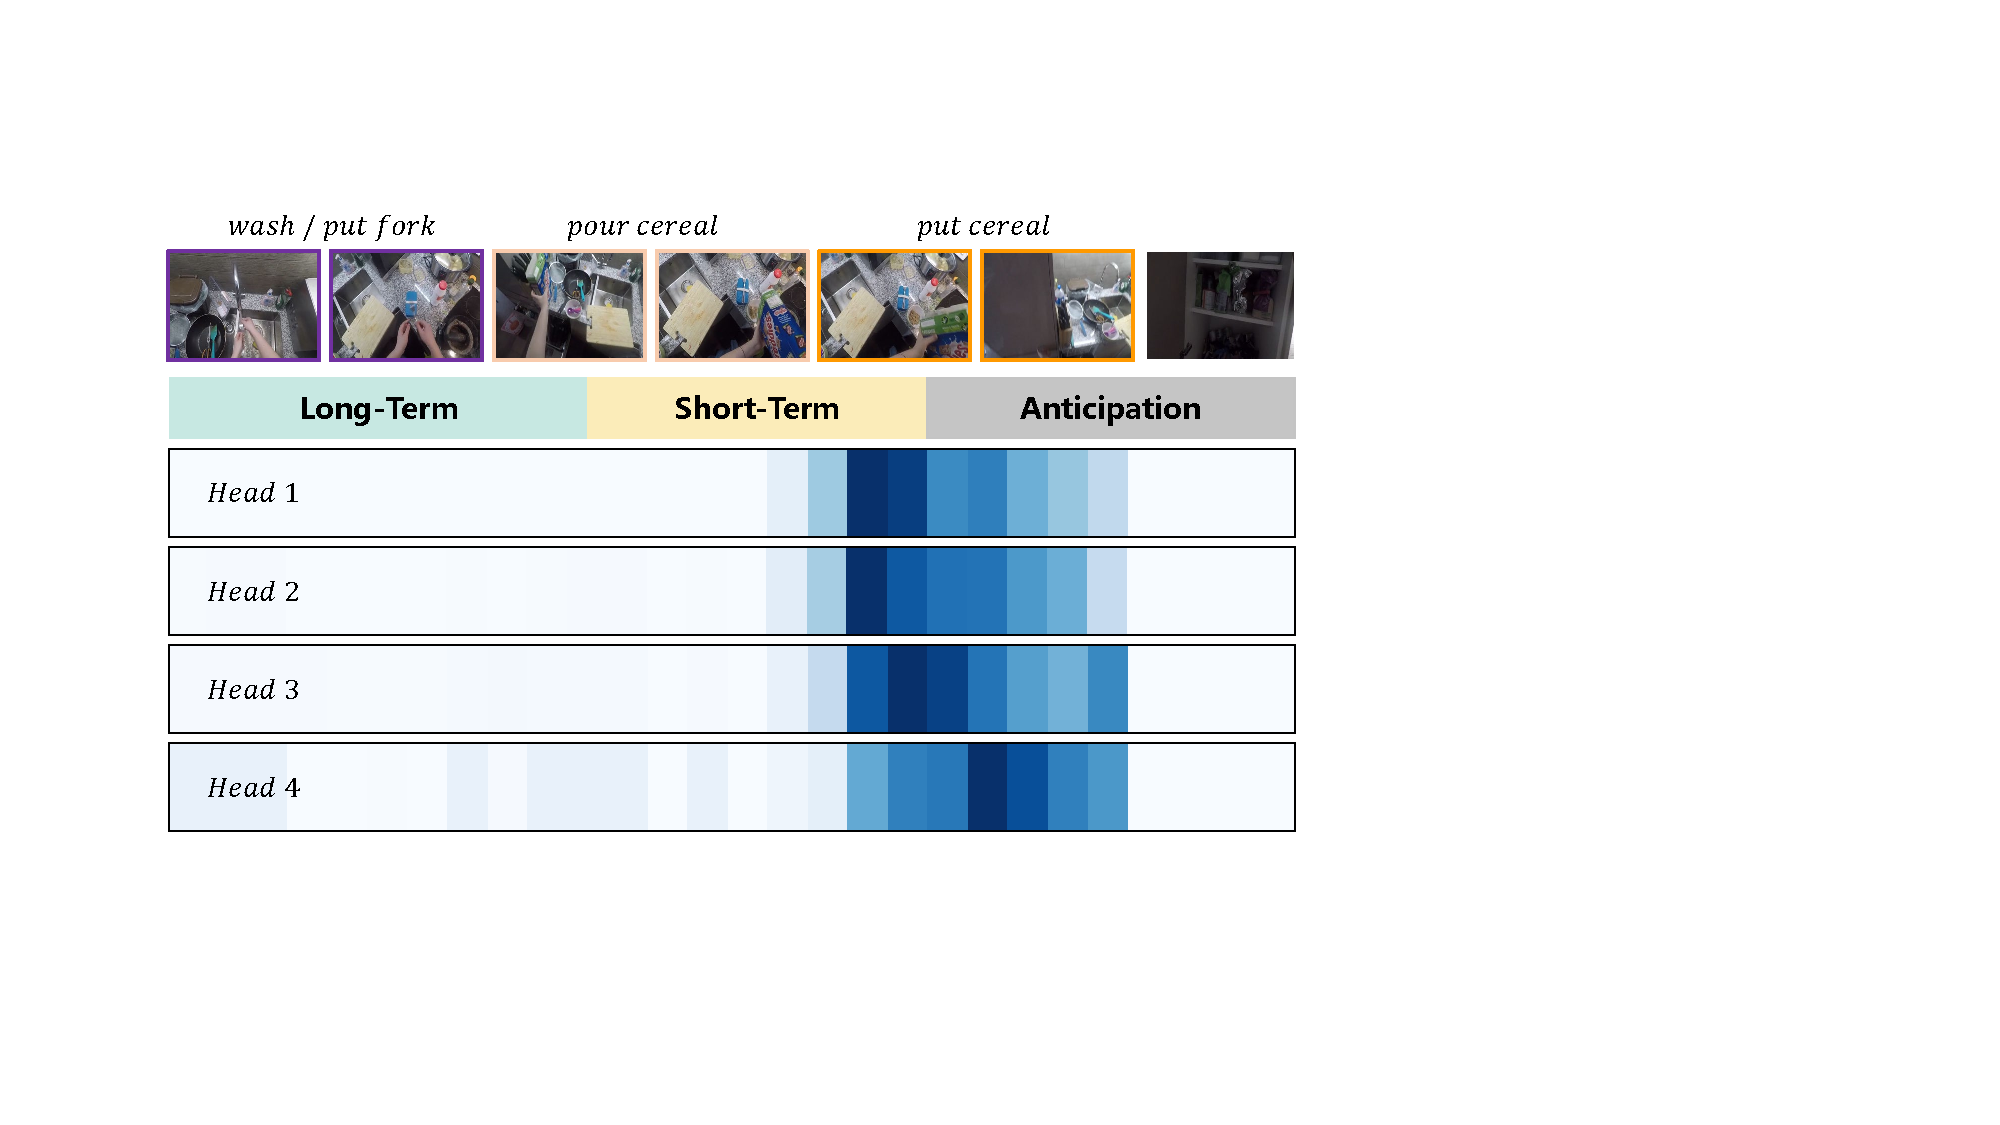
\includegraphics[width=0.48\textwidth]{images/attn_vis_single.pdf}
    \caption{\textbf{Attention weight visualization of different attention heads.}}
    \vspace{-3mm}
    \label{attn_vis}
\end{figure}

\subsection{Attention Visualization}
Fig~\ref{attn_vis} depicts the attention weights of the last token of the short-term memory. It can be seen that under the blessing of future perception, MAT's multi-head attention mechanism pays attention to memory and anticipation simultaneously, leading to the model not limiting in history and attaining better performance. 

